% !TEX TS-program = pdflatex
% !TEX encoding = UTF-8 Unicode
% !TEX root = main.tex
% !TEX spellcheck = en-US
% ****************************************************************************************
% File: thesis.tex
% Author: Patrick Haselwanter
% Date: 2023-10-28
% ****************************************************************************************
\documentclass[a4paper,11pt,oneside,final,titlepage,openany,onecolumn]{report}
% input preamble (include additional packages, set options, define macros)
% !TEX TS-program = pdflatex
% !TEX encoding = UTF-8 Unicode
% !TEX root = ../main.tex
% !TEX spellcheck = en-US
% ****************************************************************************************
% File: _preamble.tex
% Author: Patrick Haselwanter
% Date: 2023-10-28
% ****************************************************************************************

% ****************************************************************************************
% General settings (input encoding, font encoding, font, language)
% ****************************************************************************************
\usepackage[utf8]{inputenc} % character encoding used in input file
\usepackage[T1]{fontenc} % specifies the encoding used in the fonts
\usepackage{lmodern} % provides more support for non-ASCII characters than cm-super
\usepackage{microtype} % improves line-filling when using PDFLaTeX
\usepackage[ngerman,english]{babel} %  last language is considered the main one
\renewcommand{\familydefault}{\sfdefault} % select a sans serif font family 

% \pdfsuppresswarningpagegroup=1 % suppress warning when including PDFs with page groups

% ****************************************************************************************
% Basic macros for thesis
% ****************************************************************************************
\newcommand{\authorAName}{Jakob Spindler}
\newcommand{\authorAContact}{sj0458@mci4me.at}

\newcommand{\courseName}{Mobile Robotics}
\newcommand{\courseCode}{MECH-M-2-ROB}
\newcommand{\department}{Department of Technology \& Life Sciences}
\newcommand{\docTitle}{TurtlesimAutomata - dipping the toe into ROS}
\newcommand{\docType}{Software report}
\newcommand{\studyProgram}{Master's program Mechatronics \& Smart Technologies}
\newcommand{\studyYear}{MA-MECH-23-VZ}
\newcommand{\lecturerName}{Daniel McGuiness}
\newcommand{\lecturerContact}{}
\newcommand{\university}{Management Center Innsbruck}

% ****************************************************************************************
% Drawing and plotting, scientific packages, 
% ****************************************************************************************
% For use of subfigure environment
\usepackage{subcaption}

% For use of cmidrule in table environment
\usepackage{booktabs}

\usepackage{makecell}

% Handling of images
\usepackage{graphicx}
\graphicspath{{./img/}}

% Colour support
\usepackage[table]{xcolor}

% Handling of MATLAB code
\usepackage{mcode}

% Tabulars with adjustable-width columns
\usepackage{tabularx}
\usepackage{multirow}

% Sketching and importing MATLAB plots
\usepackage{pgfplots}
\usepackage{grffile}
\pgfplotsset{compat=newest}
\usetikzlibrary{plotmarks}
\usetikzlibrary{arrows.meta}
\usetikzlibrary{patterns}
\usepgfplotslibrary{patchplots}
\pgfplotsset{plot coordinates/math parser=false}
\newlength\figureheight
\newlength\figurewidth

% Typesetting electrical networks
\usepackage{circuitikz}

% scientific packages
\usepackage{amsmath}
\usepackage{amsfonts}
\usepackage{xfrac}
\usepackage{siunitx}
\AtBeginDocument{\sisetup{
		mode=match,
		unit-font-command = \mathrm,
		reset-text-family=false,
		reset-text-series=false,
		reset-text-shape=false,
		exponent-product=\cdot
	}}
\DeclareSIUnit\unity{1} % can be used for dimensionless quantities
\DeclareSIUnit\sample{Sa}
% ****************************************************************************************
% Referencing and citing
% ****************************************************************************************
% Caption settings
\usepackage[
	format=plain, % typeset as normal paragraph
	labelformat=simple, % typeset label as name and number
	labelsep=period, % caption label and text separated by period and space
	textformat=simple, % caption text typeset as is
	justification=justified, % typset caption as normal paragraph
	singlelinecheck=true, % automatically center short captions
	font=small,
	labelfont=bf, % set bold font for label
	width=.75\textwidth % set fixed width for caption
]{caption}
\captionsetup[table]{position=top}
\captionsetup[figure]{position=bottom}

% Hypertext marks (should be loaded last but before geometry)
\usepackage[hyperindex]{hyperref}
% Extension options
\hypersetup{
	colorlinks, % colours the text of links and anchors (instead of borders)
	linkcolor={blue!65!black},
	citecolor={blue!65!black},
	urlcolor={blue!65!black}
}
% PDF display and information options
\hypersetup{
	pdftitle={\docTitle},
	pdfsubject={\docType},
	pdfauthor={\authorAName},
	pdfkeywords={},
	pdfcreator={pdflatex},
	pdfproducer={LaTeX with hyperref}
}

% formatting of cross-references
\usepackage[capitalise]{cleveref}
\crefformat{equation}{(#2#1#3)}
\Crefformat{equation}{Equation~(#2#1#3)}

%matlab prettifier
\usepackage{matlab-prettifier}

% ****************************************************************************************
% Bibliography settings
% ****************************************************************************************
% template from https://www.ieee.org/conferences/publishing/templates.html
\usepackage[
	backend=biber,
	style=numeric,
	natbib=true,
	sorting=nty
]{biblatex}
%\addbibresource{C:/Users/pober/OneDrive/StudiumMaster/latex/Master.bib}
%\addbibresource{Master2.bib}
% \addbibresource{../../../../bib/mybib.bib}

% \addbibresource{C:\\Users\\pober\\OneDrive\\StudiumMaster\\latex\\Master.bib} % point BibTEX at the .bib files
% \bibliographystyle{IEEEtran} % choose the reference style
% ****************************************************************************************
% Glossary (acronyms, list of symbols) settings
% ****************************************************************************************
% \usepackage[acronym,nomain,nonumberlist,nopostdot,sort=def,toc]{glossaries}
% \renewcommand*{\glstextformat}[1]{\textcolor{black}{#1}} % make links appear black
% \newglossary[slg]{symbolslist}{syi}{syg}{List of Symbols} % define custom glossary
% \glsaddkey% define custom key
% 	{unit}% key
% 	{\glsentrytext{\glslabel}}% default value
% 	{\glsentryunit}% command analogous to \glsentrytext
% 	{\GLsentryunit}% command analogous to \Glsentrytext
% 	{\glsunit}% command analogous to \glstext
% 	{\Glsunit}% command analogous to \Glstext
% 	{\GLSunit}% command analogous to \GLStext
% \glssetnoexpandfield{unit}
% \makeglossaries % create makeindex files

% \newglossarystyle{symbolsliststyle}{%
% 	\setglossarystyle{long3col}% style based on long3col
% 	\renewenvironment{theglossary}{%
% 		\begin{longtable}{lp{\glsdescwidth}>{\arraybackslash}p{2cm}}}%
% 		{\end{longtable}}%
% 	\renewcommand*{\glossaryheader}{% change the table header
% 		\bfseries Symbol & \bfseries Description & \bfseries Unit\\\hline%
% 		\endhead}%
% 	\renewcommand*{\glossentry}[2]{% change the displayed items
% 		\glstarget{##1}{\glossentryname{##1}}% name
% 		& \glossentrydesc{##1}% description
% 		& $\glsentryunit{##1}$% unit
% 		\tabularnewline
% 	}%
% }

% ****************************************************************************************
% Page layout and headers
% ****************************************************************************************
% Specify page layout (paper name and orientation specified in document class options)
\usepackage[
	includeheadfoot, % includes the head of the page into total body
	ignoremp, % disregards marginal notes in determining the horizontal margins
	nomarginpar, % shrinks spaces for marginal notes to 0pt
	hmargin=1.5in, % left and right margin
	vmargin=1in, % top and bottom margin
	headheight=14pt %  height of header
]{geometry}

\usepackage{parskip} % helps in implementing paragraph layouts

% Header and footer settings
\usepackage{fancyhdr}
\pagestyle{fancy} % set page style to 'fancy'
\renewcommand{\chaptermark}[1]{\markboth{\thechapter.\ #1}{}}
% \renewcommand{\sectionmark}[1]{\markright{\thesection.\ #1}}
\fancyhf{} % clear all header and footer fields
\fancyhead[L]{\leftmark} % set left header location (chapter)
% \fancyhead[R]{\rightmark} % set right header location (section)
\fancyfoot[C]{\thepage} % set center footer location (page count)

% ****************************************************************************************
% Packages for testing purposes (can be deleted)
% ****************************************************************************************
\usepackage{lipsum}
\usepackage{blindtext}
\usepackage{todonotes}
% EOF
% \loadglsentries{./tex/_defns.tex}
\begin{document}
	\pagenumbering{alph}
	% !TEX TS-program = pdflatex
% !TEX encoding = UTF-8 Unicode
% !TEX root = ../main.tex
% !TEX spellcheck = en-US
% ****************************************************************************************
% File: titlepage.tex
% Author: Jakob Spindler
% Date: 2024-06-01
% ****************************************************************************************

\thispagestyle{empty}
\pdfbookmark[0]{Title page}{titlepage} % sets a PDF bookmark
\thispdfpagelabel{} %  set page number shown in the tool bar of a PDF viewer
\begin{center}
	\textbf{\Huge \university}\par
	\vspace{8ex}\par
	\textbf{\LARGE \department}\par
	\vspace{4ex}\par
	\textbf{\Large \studyProgram}\par
	\vspace{4ex}\par
	
\includegraphics[scale = 0.75]{MCI_Logo.pdf}\par
	\vspace{4ex}\par
	\textbf{\LARGE \docType}\par
	\vspace{2ex}\par
	\textbf{composed as part of the course\\[0.5ex] \courseName{} (\courseCode)}\par
	\vspace{4ex}\par
	\textbf{about}\par
	\vspace{4ex}\par
	\textbf{\LARGE \docTitle}\par
	\vspace{4ex}\par
	\textbf{from}\par
	\vspace{4ex}\par
	\textbf{\Large \href{\authorAContact}{\authorAName}}
	%\textbf{\Large \href{\authorAContact}{\authorAName}\href{\authorBContact}{\authorBName}}
\end{center}
\vspace{4ex}
\begin{tabular}{ll}
	Study program & \studyProgram\\[0.5ex]
	Year & \studyYear\\[0.5ex]
	Course & \courseName{} (\courseCode)\\[0.5ex]
	Name of lecturer & \href{\lecturerContact}{\lecturerName}\\[0.5ex]
	Submission deadline & June 16, 2024
\end{tabular}
\vfill
\begin{center}
	\today
\end{center}
%EOF
	\pagenumbering{Roman}
	\pdfbookmark[0]{\contentsname}{toc} % sets a PDF bookmark
	\tableofcontents
	\newcounter{romanpagecount}
	\setcounter{romanpagecount}{\value{page}}
	\clearpage
	\pagenumbering{arabic}

	% add content here

	% !TEX TS-program = pdflatex
% !TEX encoding = UTF-8 Unicode
% !TEX root = ../main.tex
% !TEX spellcheck = en-US
% ****************************************************************************************
% File: purpose_and_scope.tex
% Author: Patrick Haselwanter
% Date: 2023-10-28
% ****************************************************************************************
\chapter{Introduction}
\label{chapter:introduction}
The \texttt{turtlesimAutomata} package is a ROS2 (Robot Operating System) package that uses a finite state machine-like structure to control a turtle in the turtlesim environment.
It's purpose is to provide an entry-level example of a ROS2 package to acquaint the user with the basic concepts of ROS2.
The \texttt{turtlesimAutomata} package is closely intertwined with the \texttt{turtlesim} package, which is a simple simulator for a mobile robot in the shape of a turtle.

\section{Assignement}
\label[section]{section:assignment}
The assignement stated the following requirements for the \texttt{turtlesimAutomata} package:
\begin{itemize}
    \item The \texttt{turtlesimAutomata} package should work closely together with the \texttt{turtlesim} package.
    \item The turtle shall start off in a random direction
    \item The turtle shall move in a straight line until it reaches the edge of the turtlesim window, at which point it shall make a 90 degree turn in clockwise direction and continue moving in the new direction.
\end{itemize}





% EOF
	% !TEX TS-program = pdflatex
% !TEX encoding = UTF-8 Unicode
% !TEX root = ../main.tex
% !TEX spellcheck = en-US
% ****************************************************************************************
% File: package_overview.tex
% Author: Jakob Spindler
% Date: 2024-06-01
% ****************************************************************************************
\chapter{Package overview}
\label{chapter:package_overview}
The \texttt{turtlesimAutomata} package consists of the following nodes:

\begin{itemize}
    \item \texttt{/start\_turtle} listens to the \emph{/rosout} topic for a message containing "Spawning turtle" which indicates that the \texttt{turtlesim\_node} node has started successfully. It will then send a randomly computed angle to the \texttt{/turn\_turtle} node via the \emph{/turn\_angle} topic and shut itself down afterwards.
    \item \texttt{/drive\_turtle\_continuously} continuously sends a message to the \emph{/turtle1/cmd\_vel} topic to drive the turtle in a straight line. The sending of said message may be toggled via the \emph{/drive\_turtle} topic.
    \item \texttt{/turn\_turtle} listens to the \emph{/turn\_angle} topic for a message containing the angle by which the turtle shall turn. The node includes a client for the \emph{/turtle1/teleport\_relative} service (not visible in \autoref{fig:turtlesimAutomata_nodes}), which is hosted by the \texttt{/turtlesim\_node} and is being used to request a turn of the turtle by the received angle. The node functions mostly as a relay station.
    \item \texttt{/edge} listens to the \emph{/rosout} topic for a message containing "Oh no! I hit the wall!" which is published by the \texttt{turtlesim\_node} node when the turtle reaches the edge of the window. It will then tell the \texttt{/drive\_turtle\_continuously} node to stop driving the turtle forwards, send a message via the \emph{/turn\_angle} topic to request a 90 degree clockwise turn by the \texttt{/turn\_turtle} node and afterwards tells the \texttt{/drive\_turtle\_continuously} node to continue driving the turtle forwards.
\end{itemize}


\begin{figure}[htbp]
    \centering
    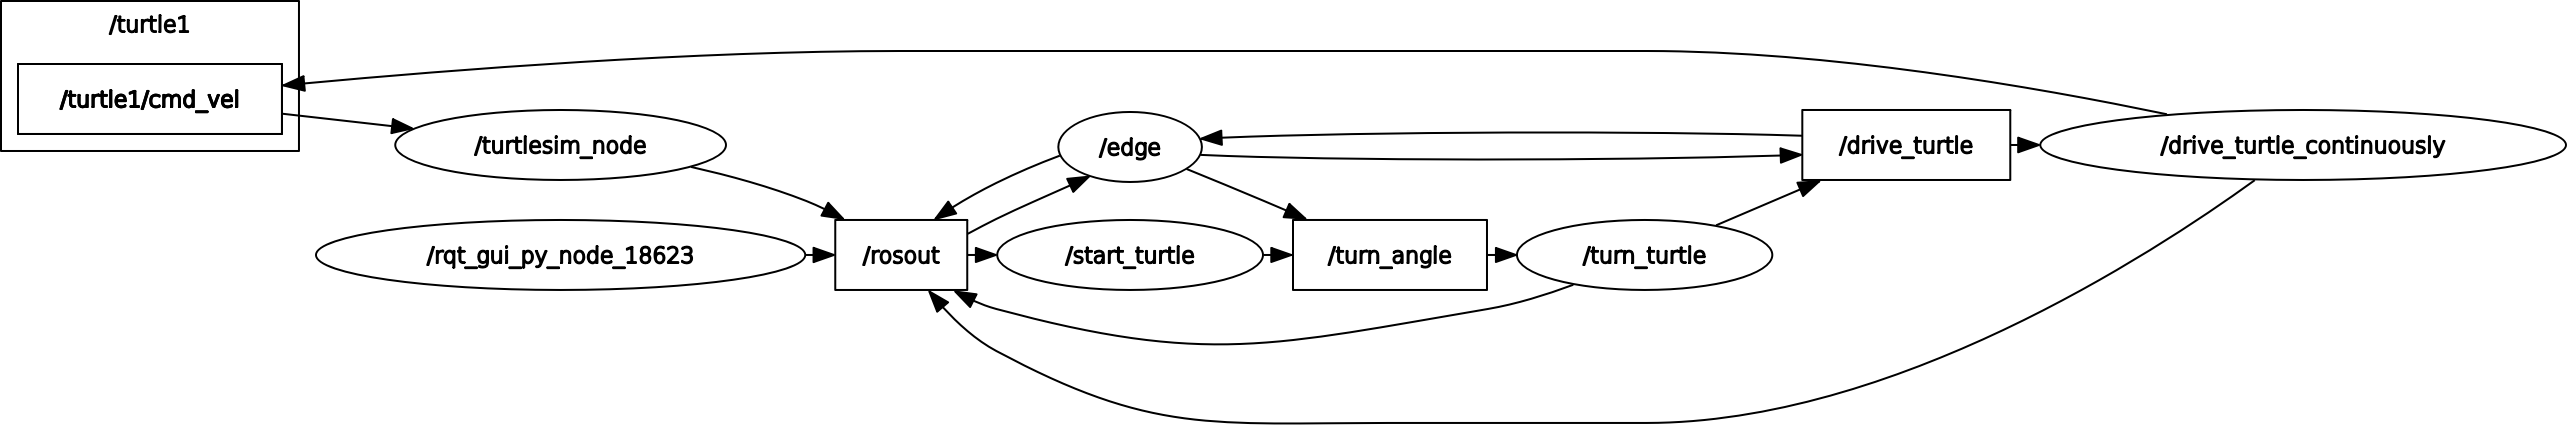
\includegraphics[width=1\textwidth]{./img/rosgraph.png}
    \caption{Nodes and topics of the \texttt{turtlesimAutomata} package shown in \texttt{rqt\_graph}}
    \label{fig:turtlesimAutomata_nodes}
\end{figure}



% EOF
	% !TEX TS-program = pdflatex
% !TEX encoding = UTF-8 Unicode
% !TEX root = ../main.tex
% !TEX spellcheck = en-US
% ****************************************************************************************
% File: behaviour.tex
% Author: Jakob Spindler
% Date: 2024-06-01
% ****************************************************************************************
\chapter{Behaviour of the turtle}
\label{chapter:behaviour_of_the_turtle}

The following \autoref{fig:turtlesim_examples_a_to_d} shows examples of the turtle's behaviour, showcasing that the \texttt{turtlesimAutomata} package is working as intended.


\begin{figure}[htbp]
    \centering
    \begin{subfigure}[b]{0.40\textwidth}
        \centering
        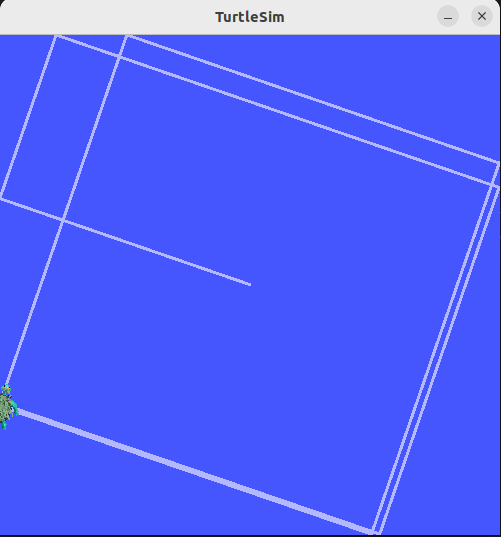
\includegraphics[width=\textwidth]{turtle_example1.png}
        \caption{}
        \label{fig:example_a}
    \end{subfigure}
    \hfill
    \begin{subfigure}[b]{0.40\textwidth}
        \centering
        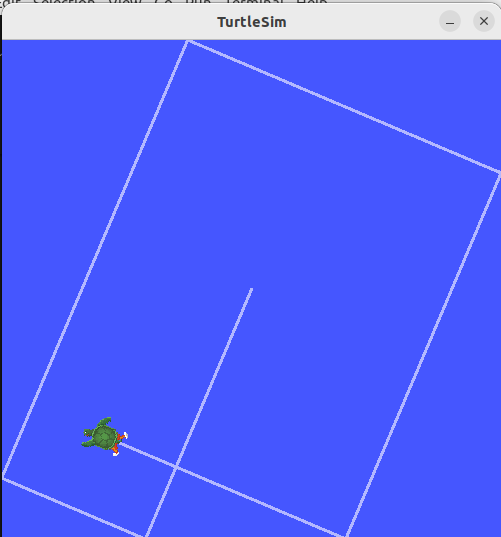
\includegraphics[width=\textwidth]{turtle_example3.png}
        \caption{}
        \label{fig:example_b}
    \end{subfigure}
\\
    \centering
    \begin{subfigure}[b]{0.40\textwidth}
        \centering
        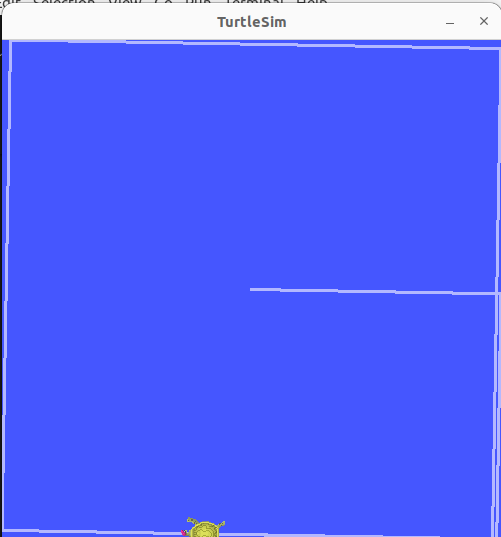
\includegraphics[width=\textwidth]{turtle_example5.png}
        \caption{}
        \label{fig:example_c}
    \end{subfigure}
    \hfill
    \begin{subfigure}[b]{0.40\textwidth}
        \centering
        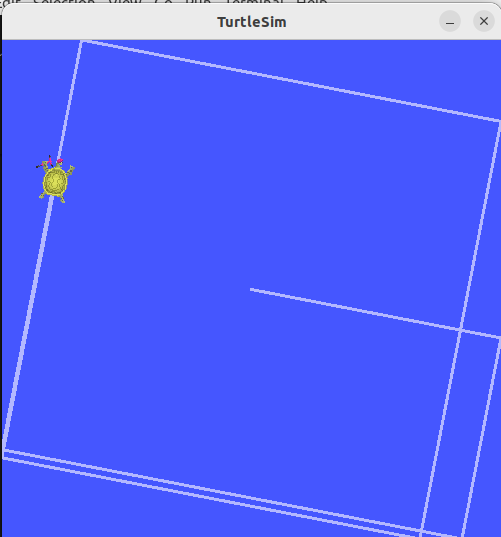
\includegraphics[width=\textwidth]{turtle_example4.png}
        \caption{}
        \label{fig:example_d}
    \end{subfigure}
    \caption{Examples of the turtle's behaviour}
    \label{fig:turtlesim_examples_a_to_d}
\end{figure}


% EOF
	% !TEX TS-program = pdflatex
% !TEX encoding = UTF-8 Unicode
% !TEX root = ../main.tex
% !TEX spellcheck = en-US
% ****************************************************************************************
% File: purpose_and_scope.tex
% Author: Patrick Haselwanter
% Date: 2023-10-28
% ****************************************************************************************
\chapter{Additional functionalities}
\label{chapter:additional_functionalities}

The \texttt{turtlesimAutomata} package can be used in combination with the \texttt{turtlesim\_teleop} package, which allows the user to manually control the turtle in the turtlesim environment, whilst still mainting the automatic behaviour provided by the \texttt{turtlesimAutomata} package. This may result in interesting behaviour, as shown in \autoref{fig:example_teleop}.

\begin{figure}[htbp]
    \centering
    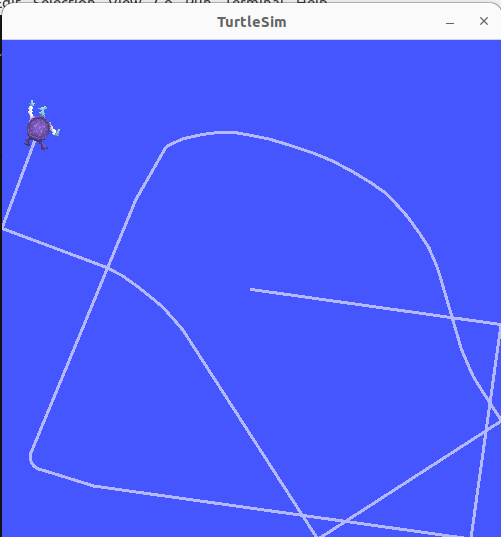
\includegraphics[width=0.4\textwidth]{./img/turtle_teleop_example.png}
    \caption{\texttt{turtlesimAutomata} and \texttt{turtlesim\_teleop} working together}
    \label{fig:example_teleop}
\end{figure}

\autoref{fig:rqt_graph_teleop} shows the \texttt{rqt\_graph} of the \texttt{turtlesimAutomata} and \texttt{turtlesim\_teleop} packages working together.

\begin{figure}[htbp]
    \centering
    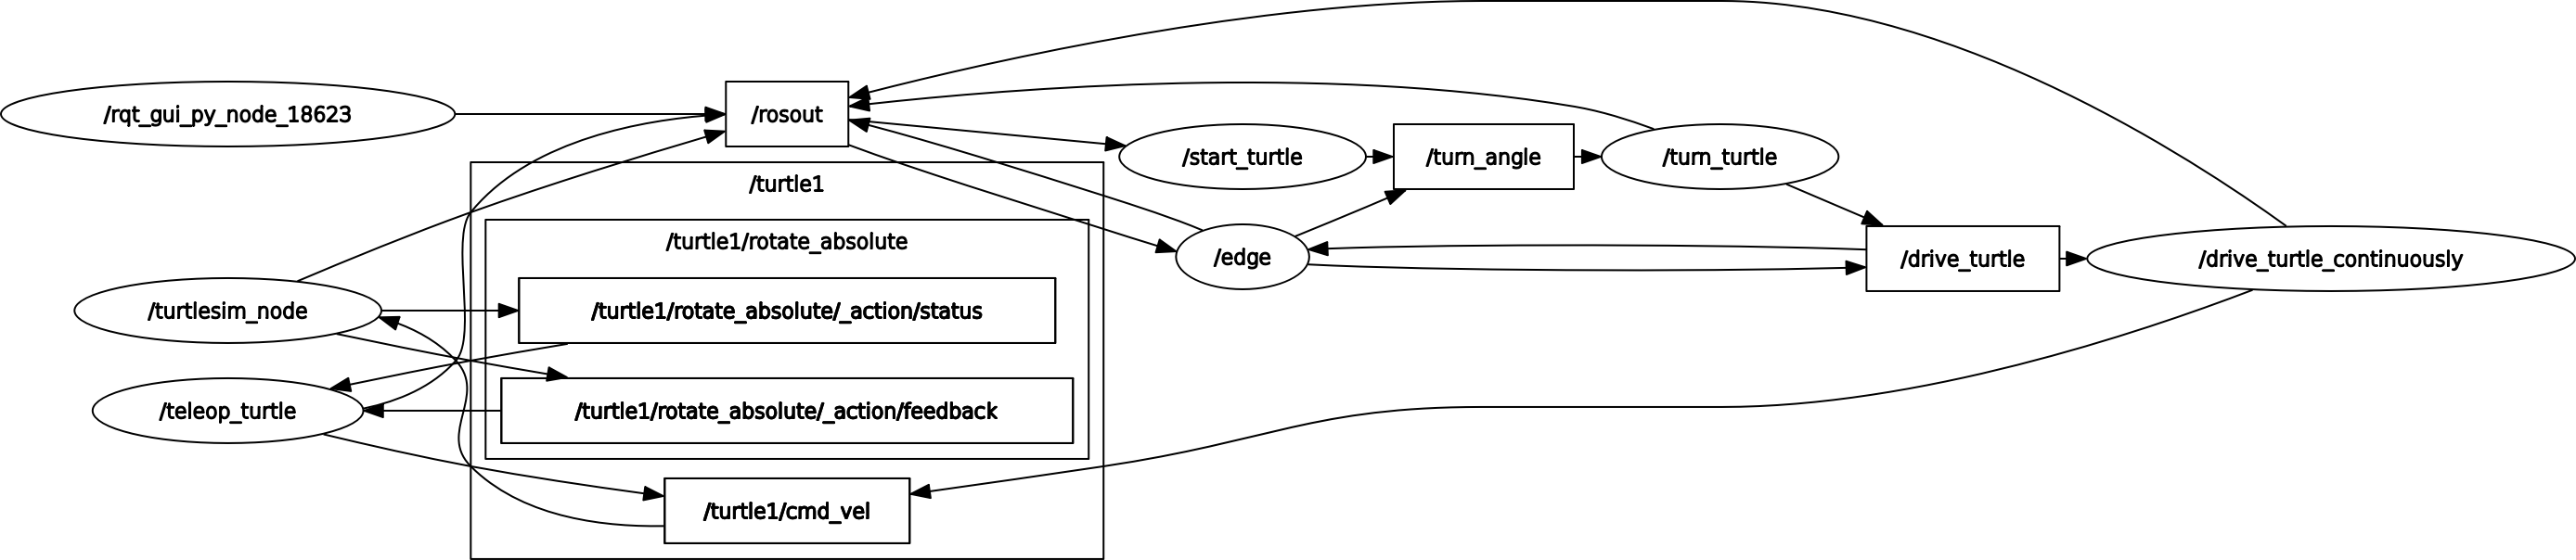
\includegraphics[width=1\textwidth]{./img/rosgraph_teleop.png}
    \caption{turtlesimAutomata and \texttt{turtlesim\_teleop} working together shown in \texttt{rqt\_graph}}
    \label{fig:rqt_graph_teleop}
\end{figure}

% EOF


	\pagenumbering{Roman}
	\setcounter{page}{\value{romanpagecount}}
	\stepcounter{page}
	\printbibliography[heading=bibintoc] % This will add the bibliography to the table of contents
	% \addcontentsline{toc}{chapter}{\bibname}
	\listoffigures
	% \addcontentsline{toc}{chapter}{\listfigurename}
	\listoftables
	% \addcontentsline{toc}{chapter}{\listtablename}
	\clearpage
	% \printglossary[type=acronym] % input files created by makeindex
	% \printglossary[type=symbolslist,style=symbolsliststyle] % input files created by makeindex

	\appendix
	% !TEX TS-program = pdflatex
% !TEX encoding = UTF-8 Unicode
% !TEX root = ../main.tex
% !TEX spellcheck = en-US
% ****************************************************************************************
% File: appendix.tex
% Author: Patrick Haselwanter
% Date: 2023-10-28
% ****************************************************************************************
\chapter{MATLAB script}
\label{chapter:MATLAB_script}

\begin{lstlisting}
    clear all
\end{lstlisting}


% EOF

\end{document}
% EOF